% ============================================================
%  Informe: Exploración y limpieza de un dataset (Protocolo EDA)
%  Seminario de Investigación II - UNSAAC
%  Compilar:  pdflatex informe_eda.tex  (x2 para referencias)
% ============================================================
\documentclass[11pt,a4paper]{article}
\usepackage[utf8]{inputenc}
\usepackage[T1]{fontenc}
\usepackage[spanish,es-tabla]{babel}
\usepackage{lmodern}
\usepackage[margin=2.3cm]{geometry}
\usepackage{graphicx}
\usepackage{booktabs}
\usepackage{tabularx}
\usepackage{xcolor}
\usepackage{float}
\usepackage{enumitem}
\usepackage{caption}
\usepackage{amssymb}
\usepackage{tikz}
\usepackage{fancyhdr}
\usepackage[hidelinks]{hyperref}

% --- paleta azul -> turquesa -> verde (coherente con la tesis) ---
\definecolor{g0}{HTML}{17365D}
\definecolor{g1}{HTML}{1F6FB2}
\definecolor{g2}{HTML}{2AA8A8}
\definecolor{g3}{HTML}{38BF8F}
\definecolor{g4}{HTML}{7FD16B}
\captionsetup{font=small,labelfont=bf,labelsep=period}
\newcommand{\paso}[1]{\colorbox{g0}{\textcolor{white}{\textbf{\,#1\,}}}}
\setlength{\parskip}{4pt}
\setlength{\parindent}{0pt}

% --- encabezado y pie institucionales ---
\pagestyle{fancy}
\fancyhf{}
\fancyhead[L]{\footnotesize\textsc{Seminario de Investigaci{\'o}n II}}
\fancyhead[R]{\footnotesize EDA \textbar\ Corpus \texttt{qxp}}
\fancyfoot[C]{\footnotesize\thepage}
\renewcommand{\headrulewidth}{0.4pt}
\renewcommand{\footrulewidth}{0pt}

\begin{document}

% ================= CAR{\'A}TULA =================
\begin{titlepage}
\centering
\thispagestyle{empty}
{\normalsize\bfseries UNIVERSIDAD NACIONAL DE SAN ANTONIO ABAD DEL CUSCO\par}
\vspace{0.30cm}
{\normalsize\bfseries FACULTAD DE INGENIER{\'I}A EL{\'E}CTRICA, ELECTR{\'O}NICA,\\ INFORM{\'A}TICA Y MEC{\'A}NICA\par}
\vspace{0.30cm}
{\normalsize\bfseries ESCUELA PROFESIONAL DE INGENIER{\'I}A INFORM{\'A}TICA Y DE SISTEMAS\par}
\vspace{0.7cm}

\IfFileExists{logo_unsaac.png}{
\includegraphics[width=3.4cm]{logo_unsaac.png}}{}
\vspace{0.7cm}

{\bfseries INFORME DE TRABAJO ENCARGADO\par}
\vspace{0.45cm}

\begin{tikzpicture}
  \node[draw=black, line width=0.6pt, rounded corners=12pt, inner sep=12pt,
        text width=0.82\linewidth, align=center, font=\bfseries\small]{%
    \textcolor{g0}{EXPLORACI{\'O}N Y LIMPIEZA DE UN DATASET DE VOZ QUECHUA}
    \textcolor{g2}{MEDIANTE EL PROTOCOLO EDA}
    \textcolor{g3}{(CORPUS COMMON VOICE \texttt{qxp})}};
\end{tikzpicture}\par
\vspace{0.6cm}

\begin{flushleft}
\hspace*{0.14\textwidth}%
\begin{minipage}{0.72\textwidth}
\raggedright\fontsize{10}{13}\selectfont
{\bfseries ASIGNATURA:}\\[3pt]
Seminario de Investigaci{\'o}n II\\[12pt]
{\bfseries PRESENTADO POR:}\\[3pt]
Br. ALAIN ARMANDO CONDORI CONTRERAS\\[3pt]
C{\'O}DIGO: 021501\\[12pt]
{\bfseries DOCENTE:}\\[3pt]
Msc. RA{\'U}L HUILLCA HUALLPARIMACHI\\[12pt]
{\bfseries SEMESTRE:} 2026-II
\end{minipage}
\end{flushleft}

\vspace{1.3cm}
{\bfseries CUSCO - PER{\'U}\par}
\vspace{0.2cm}
{\bfseries 2026\par}
\end{titlepage}

% ================= {\'I}NDICE =================
\thispagestyle{empty}
\tableofcontents
\clearpage
\setcounter{page}{1}

% ================= RESUMEN =================
\vspace{-0.2cm}

\noindent\colorbox{g4!22}{\parbox{\linewidth}{\small
\textbf{Resumen.} Se aplica el protocolo de 5 pasos y 8 herramientas del material del curso
(\emph{El Protocolo del Detective}) al subconjunto \texttt{validated} de Common Voice 27.0, variedad
quechua sureño (\texttt{qxp}), corpus base del sistema ASR de la tesis. Partiendo de
\textbf{22\,727} clips $\times$ 13 columnas, el diagnóstico revela columnas vacías, un
\textbf{desbalance severo de género}, concentración de hablantes y una estructura multi-etiqueta de
dominio; tras la limpieza se obtiene un dataset de \textbf{21\,653} filas apto para entrenar. Todo el
proceso es reproducible (\texttt{python eda\_limpieza.py}).}}

% ------------------------------------------------------------------
\section{El dataset y las variables de análisis}
El corpus \texttt{qxp} entrega, por cada clip de audio validado, su transcripción y metadatos. A las
columnas originales se añaden variables derivadas de \emph{forma del habla}, útiles para el ASR:

\begin{center}\small
\begin{tabularx}{\linewidth}{@{}l l X@{}}
\toprule
\textbf{Variable} & \textbf{Tipo} & \textbf{Significado} \\
\midrule
\texttt{dur\_s} & numérica & Duración del audio en segundos (de \texttt{clip\_durations.tsv}). \\
\texttt{n\_chars}, \texttt{n\_words} & numérica & Longitud de la transcripción (caracteres / palabras). \\
\texttt{cps} & numérica & Velocidad de habla $=$ \texttt{n\_chars}/\texttt{dur\_s} (car/s). \\
\texttt{up\_votes}, \texttt{down\_votes}, \texttt{net\_votes} & numérica & Votos de validación comunitaria. \\
\texttt{sentence\_domain} & categórica & Dominio temático (\textbf{multi-etiqueta}). \\
\texttt{age}, \texttt{gender}, \texttt{accents} & categórica & Metadatos demográficos del hablante. \\
\texttt{client\_id} & categórica & Identificador del hablante (77 en total). \\
\bottomrule
\end{tabularx}
\end{center}

% ------------------------------------------------------------------
\section{\paso{Paso 0} El Primer Vistazo}
\texttt{head()}, \texttt{info()} y \texttt{describe()} confirman \textbf{22\,727} filas y tipos
coherentes. El resumen numérico sitúa la duración media en \textbf{4,83\,s} (rango 1,8--14,9), las
frases entre 11 y 83 caracteres y la velocidad media en \textbf{7,27 car/s}. Dos columnas
(\texttt{variant}, \texttt{segment}) aparecen completamente vacías desde el inicio.

% ------------------------------------------------------------------
\section{\paso{Paso 1} La Escena del Crimen (calidad y limpieza)}

\textbf{Nulos.} La Figura~\ref{fig:nulos} mapea los faltantes. \texttt{variant} y \texttt{segment} son
\textbf{100\,\%} nulas (sin valor informativo); \texttt{accents} 63,2\,\% y \texttt{gender} 27,9\,\%.
Como son metadatos demográficos que \emph{no invalidan} el audio ni su transcripción, se opta por
marcarlos como \texttt{unknown} en lugar de borrar filas: eliminar por \texttt{accents} costaría casi
dos tercios del corpus, una pérdida injustificable para una tarea de voz.

\begin{figure}[H]
\centering
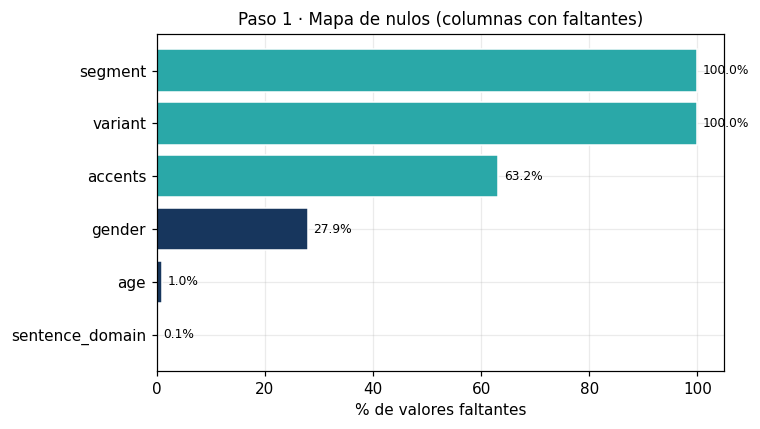
\includegraphics[width=0.72\linewidth]{figuras/fig1_nulos.png}
\caption{Porcentaje de valores faltantes por columna. En turquesa, las columnas inservibles ($\ge$50\,\%).}
\label{fig:nulos}
\end{figure}

\textbf{Duplicados.} No hay filas ni audios repetidos. Sin embargo, solo existen \textbf{2\,067 frases
únicas}: cada una se grabó $\approx$11 veces por distintos hablantes. Esto no es un defecto ---es lo
esperable en un corpus ASR multi-hablante--- pero obliga a \textbf{particionar por frase o hablante} en
el \emph{split} para evitar \emph{fuga de datos} (que una misma frase caiga en entrenamiento y prueba).

\textbf{Errores obvios.} \texttt{sentence\_domain} es multi-etiqueta (p.\,ej.\
\texttt{general,agriculture\_food,healthcare}); \textbf{76 filas} repiten tokens internos
(\texttt{healthcare,healthcare}) y se corrigen deduplicando. Ningún clip validado tiene
\texttt{net\_votes}\,$\le$\,0.

\textbf{Limpieza aplicada.} (i) Se eliminan \texttt{variant}, \texttt{segment}, \texttt{locale}
(constante) y \texttt{sentence\_id} (redundante); (ii) se normaliza el dominio en \texttt{domains},
\texttt{n\_domains} e \texttt{is\_healthcare}; (iii) los nulos demográficos pasan a \texttt{unknown};
(iv) se marcan los \emph{outliers} por regla IQR de Tukey en \texttt{dur\_s} y \texttt{cps}
(\textbf{1\,074 filas}, 4,7\,\%).

% ------------------------------------------------------------------
\section{\paso{Paso 2} Anatomía Numérica (una variable)}

Histograma y caja-y-bigotes leen los mismos datos de forma distinta: el primero muestra la
\emph{forma} de la distribución; el segundo, la mediana, la dispersión y los \emph{outliers}
(Figuras~\ref{fig:hist} y~\ref{fig:box}).

\begin{figure}[H]
\centering
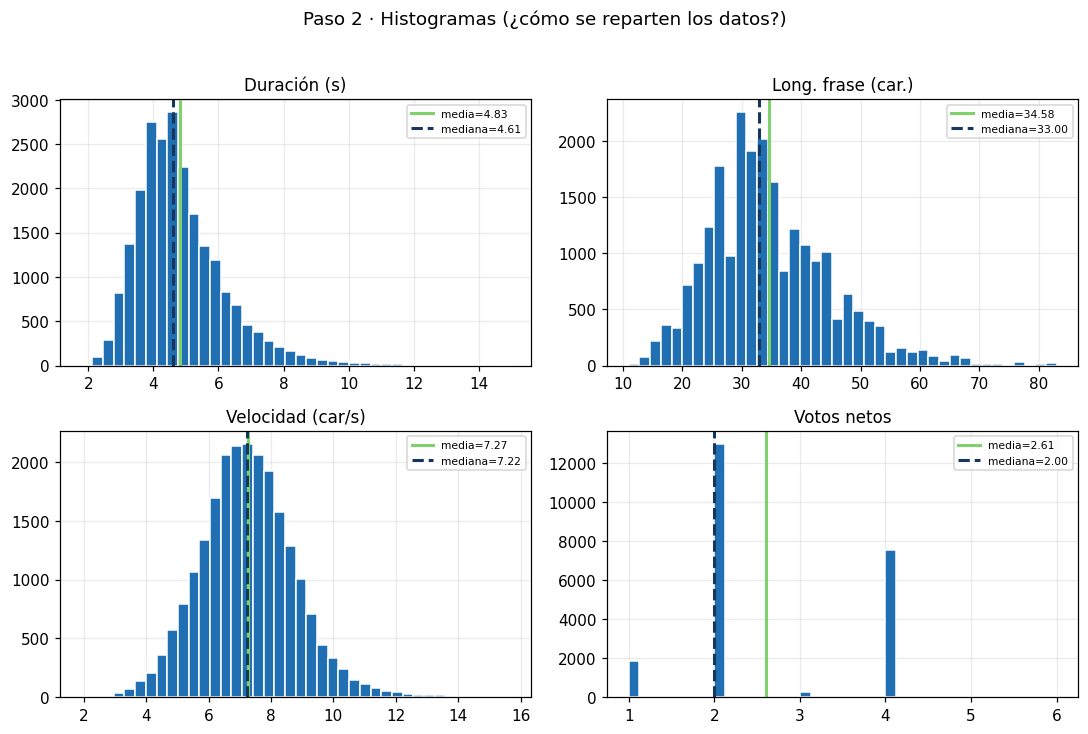
\includegraphics[width=0.82\linewidth]{figuras/fig2_histogramas.png}
\caption{Histogramas. Distribuciones unimodales, con leve asimetría a la derecha en duración y longitud.}
\label{fig:hist}
\end{figure}

\begin{figure}[H]
\centering
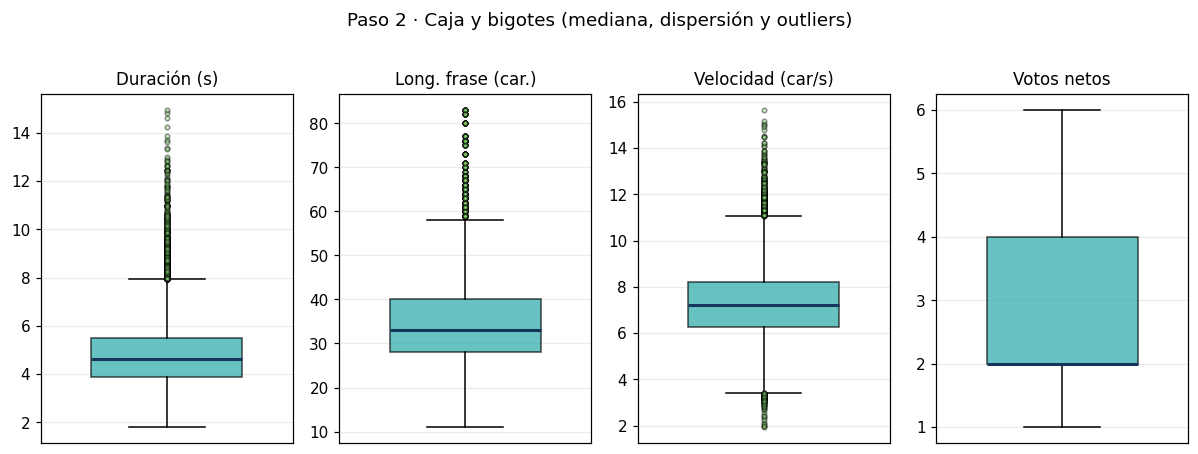
\includegraphics[width=\linewidth]{figuras/fig3_boxplots.png}
\caption{Caja y bigotes. Las colas de puntos exponen clips extremos en duración y velocidad (desajuste audio--texto).}
\label{fig:box}
\end{figure}

\textbf{El peligro del desbalance.} Las variables categóricas (Figura~\ref{fig:barras}) revelan los
hallazgos más importantes del diagnóstico:

\begin{itemize}[leftmargin=1.2em,itemsep=1pt]
  \item \textbf{Género severamente desbalanceado}: 16\,079 \texttt{female} frente a \textbf{308}
  \texttt{male} (y 6\,340 \texttt{unknown}). Un modelo entrenado así aprenderá sobre todo voz
  femenina: es un sesgo que debe declararse como limitación.
  \item \textbf{Edad} concentrada en \texttt{twenties} y \texttt{thirties}.
  \item \textbf{Dominio salud}: $\approx$\textbf{78\,\%} de los clips incluyen \texttt{healthcare},
  cobertura favorable para la tesis médica.
  \item \textbf{Concentración de hablantes}: un único hablante aporta \textbf{8,9\,\%} del corpus
  (2\,013 clips), lo que refuerza la partición por hablante.
\end{itemize}

\begin{figure}[H]
\centering
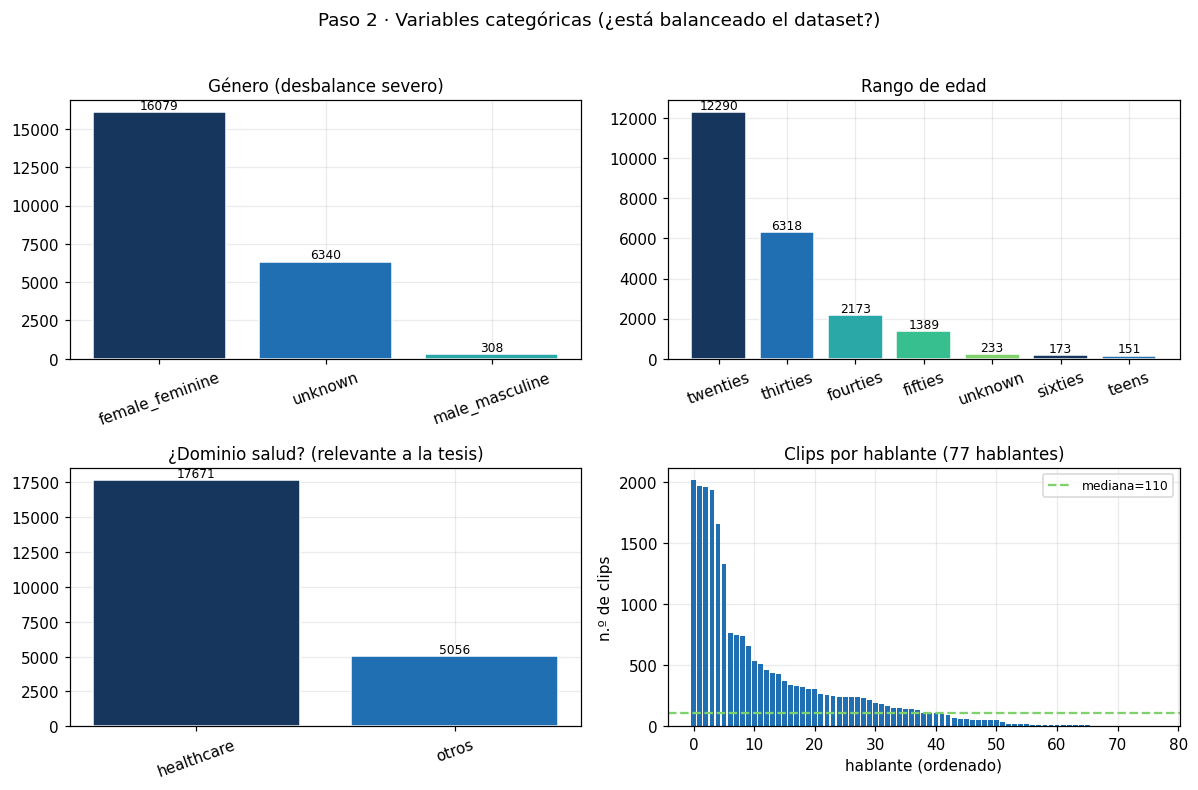
\includegraphics[width=\linewidth]{figuras/fig4_barras_categoricas.png}
\caption{Variables categóricas. El género y la concentración de hablantes son los desbalances críticos.}
\label{fig:barras}
\end{figure}

% ------------------------------------------------------------------
\section{\paso{Paso 3} Conexiones Ocultas (dos variables)}

\textbf{Dispersión.} La longitud de la frase y la duración del audio se mueven juntas en diagonal
ascendente (Figura~\ref{fig:disp}): relación \textbf{positiva} y lineal. La velocidad frente a la
duración es débilmente negativa (efecto de borde en clips muy cortos).

\begin{figure}[H]
\centering
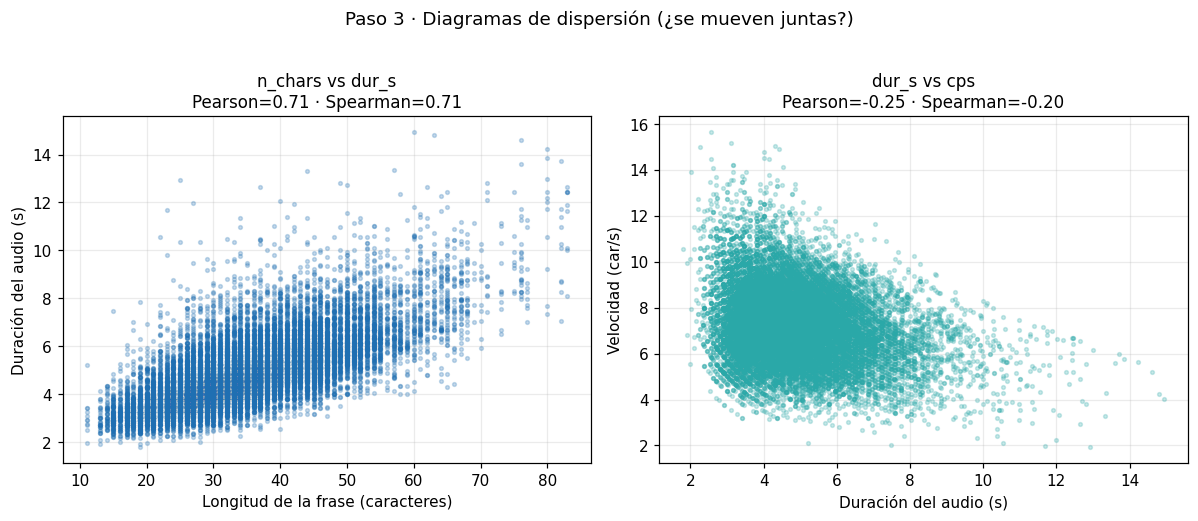
\includegraphics[width=\linewidth]{figuras/fig5_dispersion.png}
\caption{Diagramas de dispersión con sus coeficientes de Pearson y Spearman.}
\label{fig:disp}
\end{figure}

\textbf{Por qué Pearson \emph{y} Spearman.} El número puede engañar; el gráfico no. Se reportan ambos
coeficientes (Figura~\ref{fig:heat}): \textbf{Pearson} mide la asociación \emph{lineal}; \textbf{Spearman},
basado en rangos, mide la \emph{monotonía} y es robusto a \emph{outliers} y a la no-normalidad. Coinciden
en relaciones limpias (\texttt{dur\_s}\,$\sim$\,\texttt{n\_chars}\,$=0{,}71$) pero divergen donde hay
asimetría: \texttt{down\_votes}\,$\sim$\,\texttt{net\_votes} vale \textbf{$-0{,}37$} (Pearson) frente a
\textbf{$-0{,}50$} (Spearman). Esa diferencia justifica usar las dos métricas y no fiarse de una sola.

\begin{figure}[H]
\centering
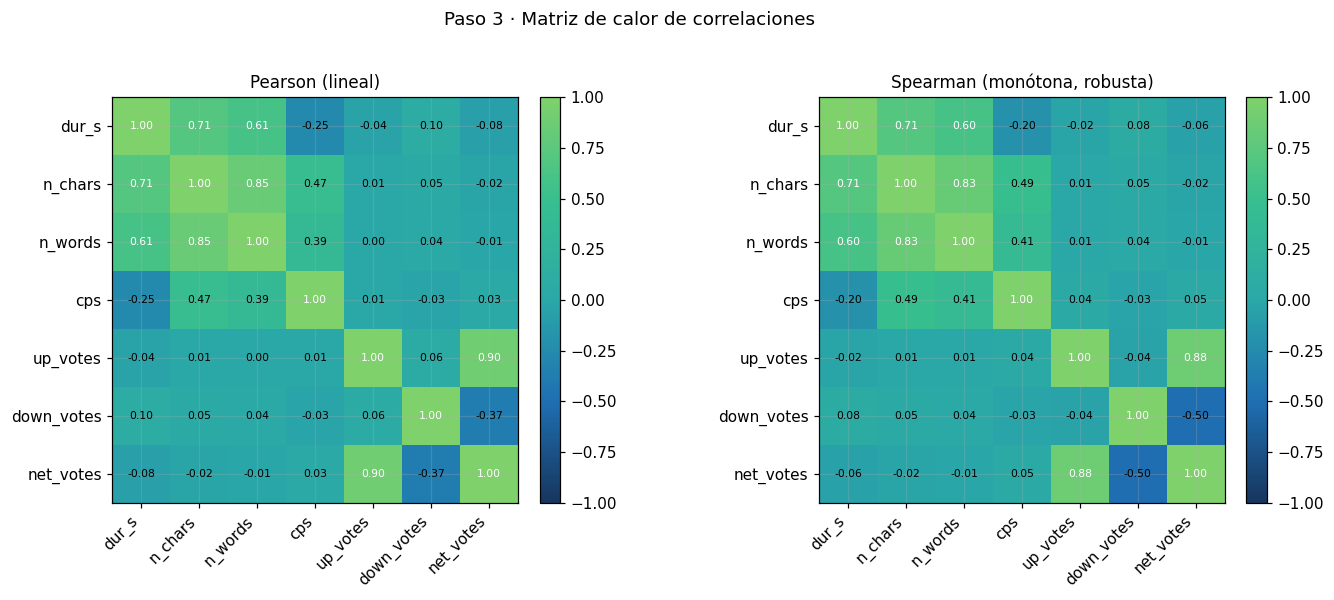
\includegraphics[width=\linewidth]{figuras/fig6_heatmaps.png}
\caption{Matrices de calor de correlación. Izq.: Pearson (lineal). Der.: Spearman (monótona, robusta).}
\label{fig:heat}
\end{figure}

% ------------------------------------------------------------------
\section{\paso{Paso 4} La Variable Objetivo}

Para la tesis, el eje de interés es \texttt{is\_healthcare}. Al cruzar las variables de forma por este
objetivo (Figura~\ref{fig:obj}), el subconjunto de salud muestra frases algo más cortas (mediana 32 vs
36 caracteres) y ligeramente más lentas. Las diferencias son pequeñas en magnitud pero
\textbf{estadísticamente significativas} (prueba de Mann--Whitney, $p \ll 0{,}001$) por el gran tamaño
muestral. Interpretación: el dominio clínico está bien representado y es homogéneo con el resto del
corpus, sin sesgos de forma que dificulten el ajuste.

\begin{figure}[H]
\centering
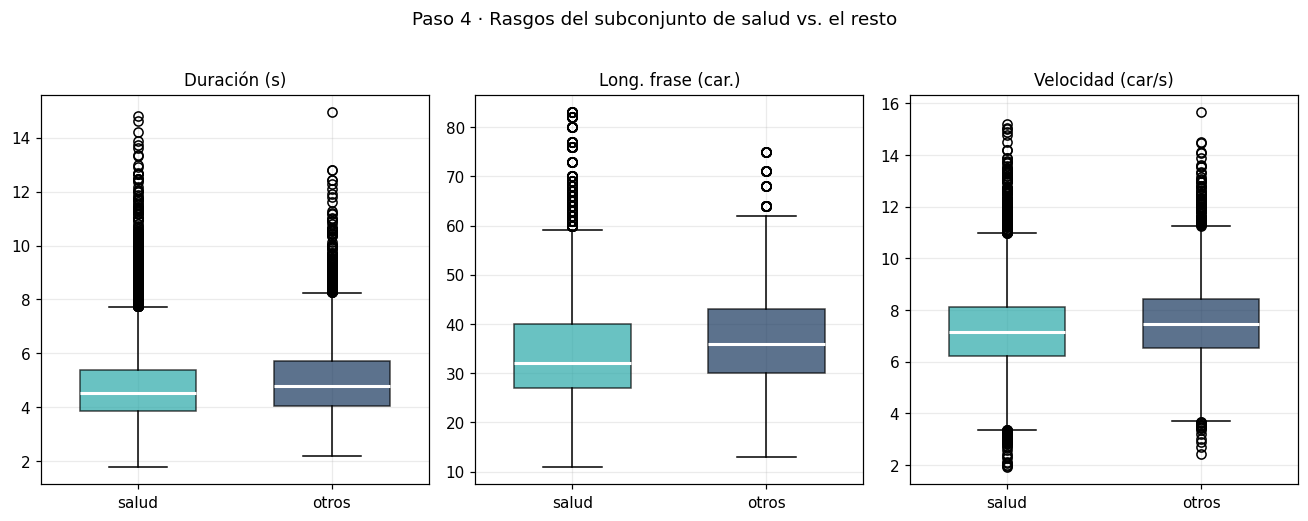
\includegraphics[width=\linewidth]{figuras/fig7_objetivo.png}
\caption{Gráficos cruzados: rasgos del subconjunto de salud frente al resto del corpus.}
\label{fig:obj}
\end{figure}

% ------------------------------------------------------------------
\section{Veredicto final: dataset limpio}
Aplicando el orden del protocolo ---primero limpiar, luego una variable, luego dos, al final el
objetivo--- se obtiene el dataset depurado. Criterio de inclusión para entrenamiento: sin
\emph{outlier} IQR (\texttt{dur\_s}, \texttt{cps}) y \texttt{net\_votes}\,$>$\,0.

\begin{center}\small
\begin{tabularx}{\linewidth}{@{}X r@{}}
\toprule
\textbf{Decisión de limpieza} & \textbf{Efecto} \\
\midrule
Eliminar columnas vacías/constantes/redundantes & $-4$ columnas \\
Normalizar \texttt{sentence\_domain} (dedup. de tokens) & 76 filas corregidas \\
Imputar nulos demográficos como \texttt{unknown} & 0 filas perdidas \\
Excluir \emph{outliers} IQR de duración y velocidad & $-1\,074$ filas (4,7\,\%) \\
\midrule
\textbf{Corpus validado crudo} $\rightarrow$ \textbf{dataset limpio} & \textbf{22\,727 $\rightarrow$ 21\,653} \\
\bottomrule
\end{tabularx}
\end{center}

% ------------------------------------------------------------------
\section{Rigurosidad del estudio}
\begin{description}[leftmargin=0pt,itemsep=2pt]
  \item[\textcolor{g0}{Metodológica.}] Se respeta el orden estricto del protocolo (Pasos 0--4). Cada
  decisión de limpieza se sustenta en evidencia numérica (porcentaje de nulos, conteo de duplicados,
  cercos IQR), no en supuestos.
  \item[\textcolor{g0}{Teórica.}] Las correlaciones se evalúan con Pearson y Spearman de forma
  complementaria (lineal vs.\ monótona/robusta); los \emph{outliers} se detectan con la regla IQR de
  Tukey; los contrastes por objetivo usan Mann--Whitney (no paramétrico), adecuado a distribuciones
  asimétricas.
  \item[\textcolor{g0}{Interpretativa.}] Toda figura va acompañada de su lectura, distinguiendo
  hallazgos reales (desbalance de género, concentración de hablantes, fuga potencial por frases
  repetidas) de asociaciones triviales (\texttt{up\_votes}\,$\sim$\,\texttt{net\_votes}).
  \item[\textcolor{g0}{Replicabilidad.}] Semilla fija (\texttt{SEED=42}), versiones de librerías
  registradas en la salida, rutas autodescubiertas y resultados deterministas. El informe, el notebook
  (\texttt{eda\_limpieza.ipynb}) y el dataset limpio se regeneran con \texttt{python eda\_limpieza.py}.
\end{description}

\vspace{4pt}
\noindent\rule{\linewidth}{0.4pt}\\[-2pt]
{\footnotesize Archivos de la entrega: \texttt{eda\_limpieza.py} (script), \texttt{eda\_limpieza.ipynb}
(notebook ejecutado), \texttt{figuras/} (7 figuras), \texttt{dataset\_limpio.csv} (21\,653 filas),
\texttt{resumen\_eda.txt} (bitácora) y este informe.}

\end{document}
